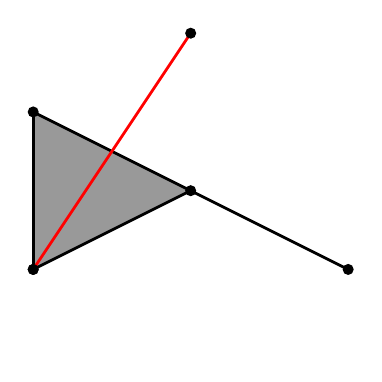
\begin{tikzpicture}[>=latex, line width=1pt]
  % Coords
  \coordinate (V0) at (2,0);
  \coordinate (V1) at (2,2);
  \coordinate (V2) at (0,1);
  \coordinate (V3) at (4,1);
  \coordinate (V4) at (4,-1);
  \coordinate (V5) at (0,-1);
 \coordinate (V6) at (2,-2);
  % Arrows\tilde{\sigma}
  \draw[opacity=0] (V0) -- (V1);
  \draw[opacity=0](V1) --  (V2);
  \draw (V0) -- (V2);
  \draw[opacity=0](V1) --  (V3);
  \draw[opacity=0](V0) -- (V3);
   \draw(V0) -- (V4);
  \draw[opacity=1](V0) -- (V5);
  \draw[opacity=1](V5) --  (V2);
  \draw[opacity=0](V3) --  (V4);
 \draw[opacity=0](V4) -- (V6);
\draw[opacity=0](V0) -- (V6);
\draw[opacity=0](V6) -- (V5);
  % Points
  \fill (V0) circle (2pt);
  \fill[opacity=0] (V1) circle (2pt);
  \fill(V2) circle (2pt);
  \fill[opacity=0] (V3) circle (2pt);
  \fill[opacity=1](V4) circle (2pt);
  \fill[opacity=1] (V5)circle (2pt);
 \fill[opacity=0] (V6)circle (2pt);

%\fill[opacity=0.4]  (V1) -- (V3) -- (V4) -- (V6) -- (V5) -- (V2);

%\draw[opacity=0] (V5) -- (V4);

\fill[opacity=0.4]  (V2) -- (V0) -- (V5);
\draw[red] (V1) -- (V5);
 \fill(V1) circle (2pt);
\fill(V5) circle (2pt);
  %circumcenter
  %\coordinate (CC1) at (1.333,1);
  %\coordinate (CC0) at (2.666,1);
  %\coordinate (CC2) at (0.666,0);
  %\coordinate (CCm) at (3.333,0);
  %\coordinate (CCC0) at (2,1);
  %\coordinate (CCC1) at (1,0.5);
  %\coordinate (CCC2) at (3,0.5);
  %\coordinate (CCC3) at (1,-0.5);
  %\coordinate (CCC4) at (3,-0.5);
 % \fill (CC0) circle (2pt);
  %\fill (CC1) circle (2pt);
  %\fill (CC2) circle (2pt);
  %\fill (CCm) circle (2pt);
  %\fill (CCC0) circle (2pt);
  %\fill (CCC1) circle (2pt);
  %\fill (CCC2) circle (2pt);
  %\fill (CCC3) circle (2pt);
  %\fill (CCC4) circle (2pt);
  %\draw[line width=1pt, ->,style=dotted] (CC0) -- (CC1);
  %\draw[line width=1pt, ->,style=dotted] (CC1) -- (CC2);
 % \draw[line width=1pt, ->,style=dotted] (CCm) -- (CC0);
 % \draw[line width=1pt,style=dotted] (CC2) -- (CCC3);
 % \draw[line width=1pt,->,style=dotted] (CCC4) -- (CCm);

\end{tikzpicture}

